\section{基于对极几何算法的相机位姿估计}

\par 对极几何是计算机视觉和立体视觉领域的一个基本概念,它描述了两个相机之间的基本几何关系,
可以用来表示三维空间中的某个点在两张图像上的投影点之间的几何约束关系。

\begin{figure}[htb]
	\centering
	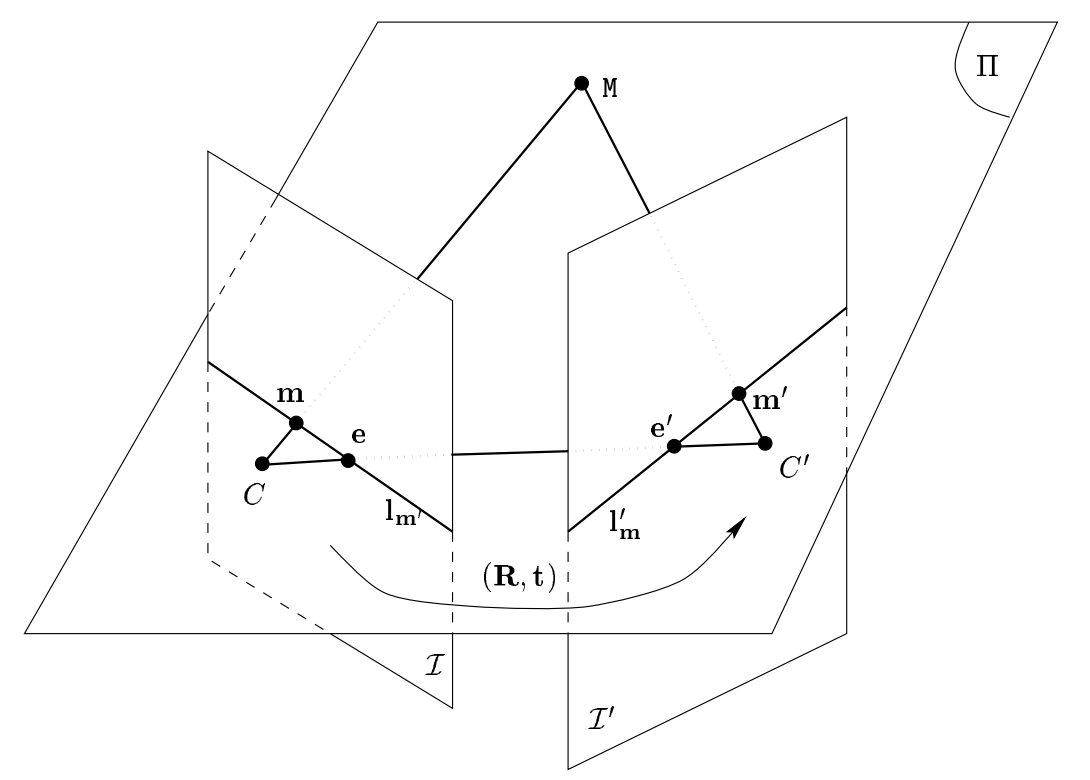
\includegraphics[width=0.7\textwidth]{figures/epipolar.png}
	\caption{对极几何示意图}
	\note{注:两个相机从不同位置观察同一三维点时,形成的对极平面、对极线以及基线。}
	\label{fig:epipolar}
\end{figure}

\par 如图\ref{fig:epipolar}\cite{epipolar}所示,有两个相机,一个在位置$C$,另一个在位置$C'$。它们都观察到了
同一个三维点$M$。$C$和$M$之间的连线与$C'$和$M$之间的连线交于$C$和$C'$之间的连线,这条线
称为基线(Baseline)。现在,可以在两个相机的图像平面上找到与$M$对应的两个二维点$m$
和$m'$。$m$,$m'$,$C$和$C'$共面,这个平面被称为对极平面(epipolar plane)。对极平面与
图像平面的交线被称为对极线(Epipolar Line),这条线包含了三维点$M$可能在图像上投影的所有位
置。这就是对极约束(Epipolar Constraint)。

\par 对极几何为估计相机的位姿提供了理论基础。利用它可以估计两个相机之间的相对位姿,
这是重建三维场景的关键步骤。利用对极约束,可以通过以下公式来估计相机的位姿:
\begin{equation}
	m'^T F m = 0
\end{equation}
\par 其中,$F$是基本矩阵(Fundamental Matrix),它封装了两个相机之间的相对位姿,$m$和$m'$是
对应的图像点。可以通过八点法或者随机采样一致性算法(Random Sample Consensus,RANSAC)等方法求解。一旦计算出$F$,就可以通过奇异值分解
(Singular Value Decomposition,SVD)来恢复旋转矩阵$R$和平移向量$t$:
\begin{align}
	F     & = K'^{-T} [t]_x R K^{-1} \\
	[t]_x & =
	\begin{bmatrix}
		0    & -t_z & t_y  \\
		t_z  & 0    & -t_x \\
		-t_y & t_x  & 0
	\end{bmatrix}
\end{align}
\par 其中,$K$和$K'$是相机的内参矩阵,$[t]_x$是$t$的反对称矩阵。
\par 最后,可以通过三角测量(Triangulation)恢复三维点$M$的坐标。

% \par 以上公式对应的是理想情况。然而,在实际应用中,需要考虑噪声和误差。因此,通常会使用
% 优化方法,比如使用最小二乘法(Least Squares)或者 Bundle Adjustment 来精细化位姿估计和
% 三维点的坐标。

% \par 对极几何是摄像机位姿估计的基础,然而它也有自身的局限性,比如不能处理在单一视图中的
% 旋转,即单应性问题。面对这个问题,可以使用比对极几何更具有普遍性的几何模型——多视几何(multiview
% geometry)。

% \par 多视几何可以处理三个或更多的视图,从而利用更多的信息来提高重建的质量和稳定性。关键概念是利用投影矩阵(projection matrix) $P$,将三维点$M$映射到二维图像点$m$:

% \begin{equation}
% 	m = P M
% \end{equation}

% \par 其中,$P$是$4 \times 3$矩阵,包含相机的内参,旋转,和平移,可以分解为三部分:

% \begin{equation}
% 	P = K [R|t]
% \end{equation}

% \par 其中,$K$是相机内参矩阵,$R$是旋转矩阵,$t$是平移向量。
% 多视几何的基本概念如图\ref{fig:multiview_geometry}所示。在实际应用中,位姿估计通常被看作是一个优化问题。
% 给定一组匹配的图像点,需要是找到最小化重投影误差的相机位姿。
% 重投影误差由真实的图像点和通过相机投影后的三维点在图像平面上的位置之间的欧几里得距离来定义。具体公式如下:

% \begin{equation}
% 	minimize \sum_{i} ||m_i - P M_i||^2
% \end{equation}

% \par 其中,$m_i$是观察到的图像点,$M_i$是对应的三维点,$P$是投影矩阵。这是一个非线性最
% 小二乘问题,可以通过 Levenberg-Marquardt\cite{Levenberg-Marquardt} 算法或者 Bundle Adjustment\cite{BundleAdjustment} 来求解。

% \begin{figure}[htb]
% 	\centering
% 	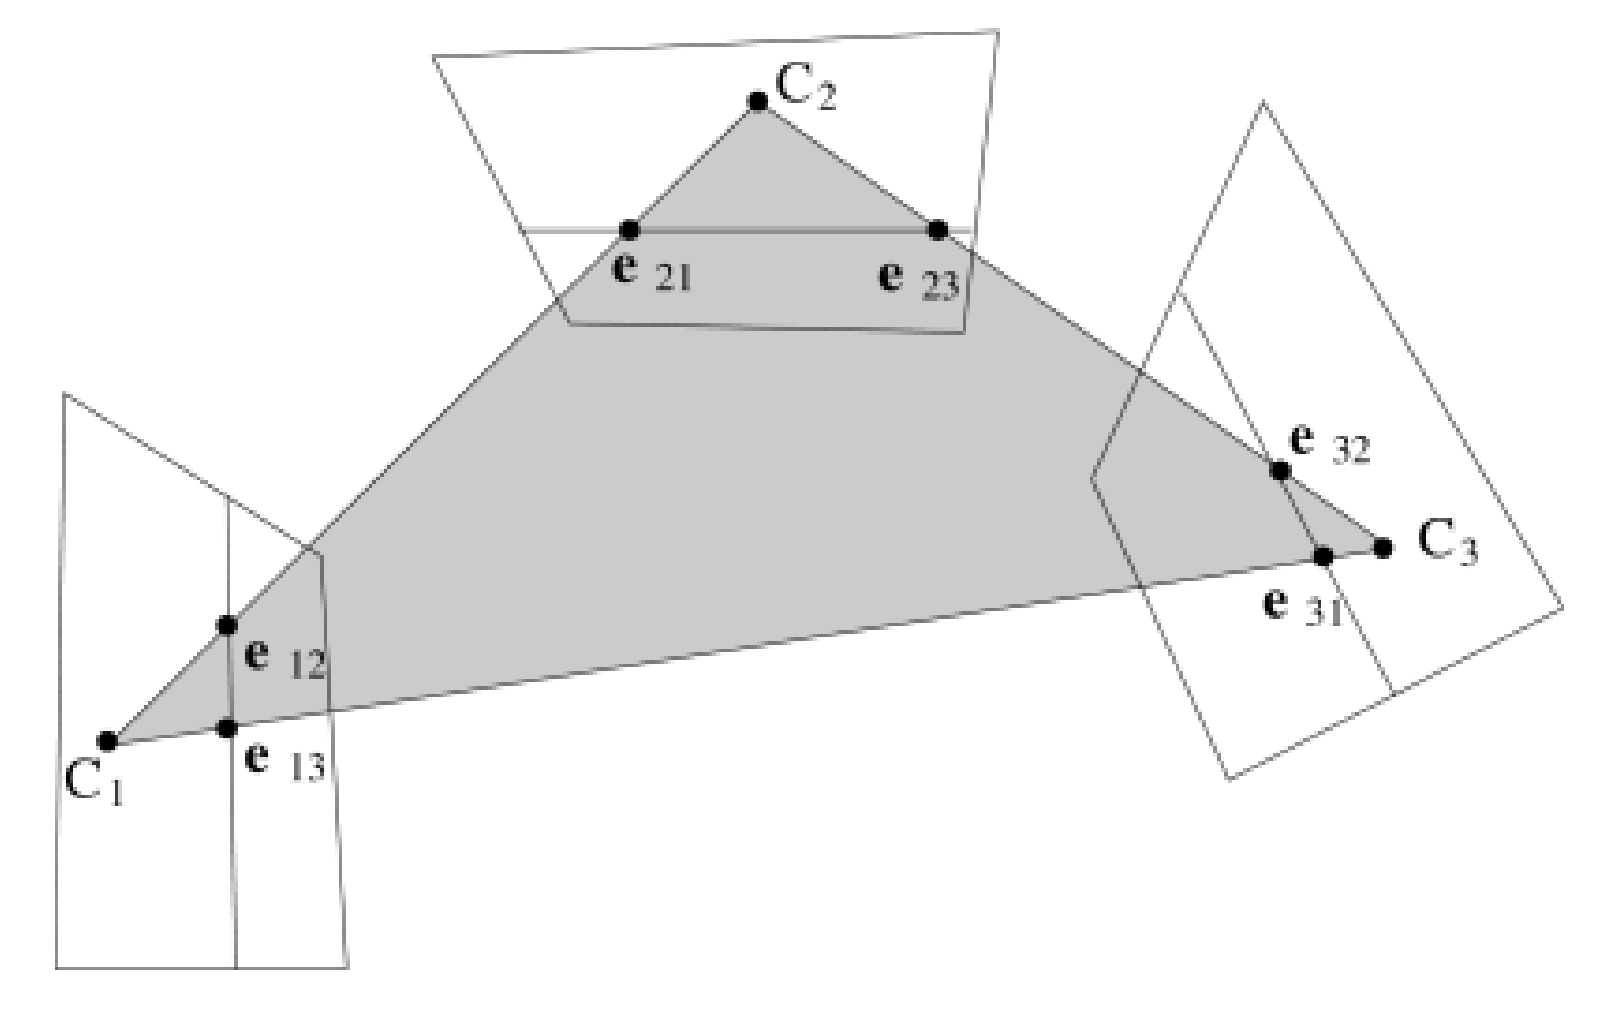
\includegraphics[width=0.7\textwidth]{figures/multiview_geometry.png}
% 	\caption{多视几何示例}
% 	\label{fig:multiview_geometry}
% \end{figure}

\par 在基于RGB-D 相机的三维重建中,RGB-D相机提供了额外的深度信息,这极大地简化了位姿估计
和三维重建的问题。利用深度信息,可以直接获得初始的三维点,然后通过优化位姿来提高重建的质量。